\chapter{Virtual Memory and Interprocess Communication}

\epigraph{Abbott: Now you've got it. \\
Costello: I throw the ball to Naturally. \\
Abbott: You don't! You throw it to Who! \\
Costello: Naturally. \\
Abbott: Well, that's it - say it that way. \\
Costello: That's what I said.}{Abbott and Costello on Effective Communication}

In very simple embedded systems and early computers, processes directly access memory -- ``Address 1234'' corresponds to a particular byte stored in a particular part of physical memory.
For example, the IBM 709 had to read and write directly to tape with no level of abstraction \cite[P. 65]{ibm709}.
Even in systems after that, it was hard to adopt virtual memory because virtual memory required the whole fetch cycle to be altered through hardware -- a change many manufacturers still thought was expensive.
In the PDP-10, a workaround was used by using different registers for each process and then virtual memory was added later \cite{ricm}.
In modern systems, this is no longer the case.
Instead, each process is isolated, and there is a translation process between the address of a particular CPU instruction or piece of data of a process and the actual byte of physical memory (``RAM'').
Memory addresses no longer map to physical addresses
The process runs inside virtual memory.
Virtual memory not only keeps processes safe because one process cannot directly read or modify another process's memory.
Virtual memory also allows the system to efficiently allocate and reallocate portions of memory to different processes.
The modern process of translating memory is as follows.

\begin{enumerate}
\item A process makes a memory request
\item The circuit first checks the Translation Lookaside Buffer (TLB) if the address page is cached into memory. It skips to the reading from/writing to phase if found otherwise the request goes to the MMU.
\item The Memory Management Unit (MMU) performs the address translation. If the translation succeeds, the page gets pulled from RAM -- conceptually the entire page isn't loaded up. The result is cached in the TLB.
\item The CPU performs the operation by either reading from the physical address or writing to the address.
\end{enumerate}

\section{Translating Addresses}

The Memory Management Unit is part of the CPU, and it converts a virtual memory address into a physical address.
First, we'll talk about what the virtual memory abstraction is and how to translate addresses

To illustrate, consider a 32-bit machine, meaning pointers are 32-bits.
They can address $2^{32}$ different locations or 4GB of memory where one address is one byte.
Imagine we had a large table for every possible address where we will store the `real' i.e. ~physical address.
Each physical address will need 4 bytes -- to hold the 32-bits.
Naturally, This scheme would require 16 billion bytes to store all of the entries.
It should be painfully obvious that our lookup scheme would consume all of the memory that we could possibly buy for our 4GB machine.
Our lookup table should be smaller than the memory we have otherwise we will have no space left for our actual programs and operating system data.
The solution is to chunk memory into small regions called `pages' and `frames' and use a lookup table for each page.

\subsection{Terminology}

A \textbf{page} is a block of virtual memory.
A typical block size on Linux is 4KiB or $2^{12}$ addresses, though one can find examples of larger blocks.
So rather than talking about individual bytes, we can talk about blocks of 4KiBs, each block is called a page.
We can also number our pages (``Page 0'' ``Page 1'' etc). Let's do a sample calculation of how many pages are there assume page size of 4KiB.

For a 32-bit machine,

\[
   2^{32} \text{address} / 2^{12} \text{(address/page)} = 2^{20} \text{pages}.
\]

For a 64-bit machine,

\[
   2^{64} \text{address} / 2^{12} \text{(address/page)} = 2^{52} \text{pages} \approx 10^{15} \text{pages}.
\]

We also call this a \textbf{frame} or sometimes called a `page frame' is a block of \emph{physical memory} or RAM -- Random Access Memory.
A frame is the same number of bytes as a virtual page or 4KiB on our machine.
It stores the bytes of interest.
To access a particular byte in a frame, an MMU goes from the start of the frame and adds the offset -- discussed later.

A \textbf{page table} is a map from a number to a particular frame.
For example Page 1 might be mapped to frame 45, page 2 mapped to frame 30.
Other frames might be currently unused or assigned to other running processes or used internally by the operating system.
You can imagine a page table just as that

\begin{figure}[H]
  \centering
  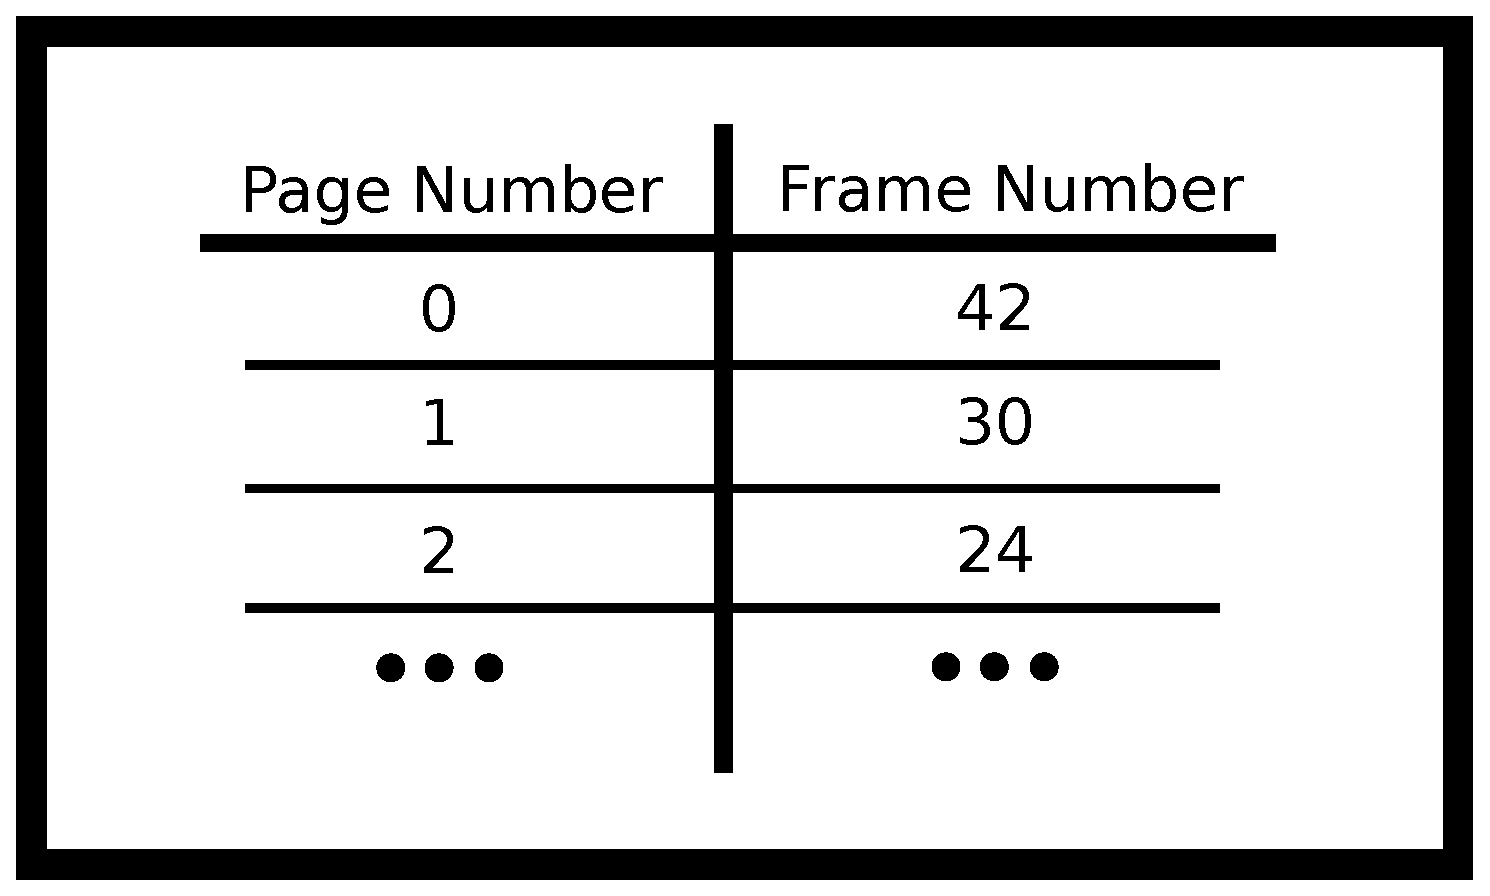
\includegraphics[width=.5\textwidth]{ipc/drawings/frame_table.eps}
  \caption{Explicit Frame Table}
\end{figure}

In practice, we will omit the first column because it will always be sequentially 0, 1, 2, etc and instead we'll use the offset from the start of the table as the entry number.

Now to go through the actual calculations.
We will assume that a 32-bit machine has 4KiB pages
Naturally to address all the possible entries, there are $2^{20}$ frames.
Since there are $2^{20}$ possible frames, we will need 20 bits to number all of the possible frames meaning \keyword{Frame Number} must be 2.5 bytes long.
In practice, we'll round that up to 4 bytes and do something interesting with the rest of the bits.
With 4 bytes per entry x $2^{20}$ entries = 4 MiB of physical memory are required to hold the entire page table for a process.

Remember our page table maps pages to frames, but each frame is a block of contiguous addresses.
How do we calculate which particular byte to use inside a particular frame?
The solution is to re-use the lowest bits of the virtual memory address directly.
For example, suppose our process is reading the following address- \keyword{VirtualAddress = 11110000111100001111000010101010 (binary)}

So to give an example say we have the virtual address above.
How would we split it up using a one-page table to frame scheme?

\begin{figure}[H]
\centering
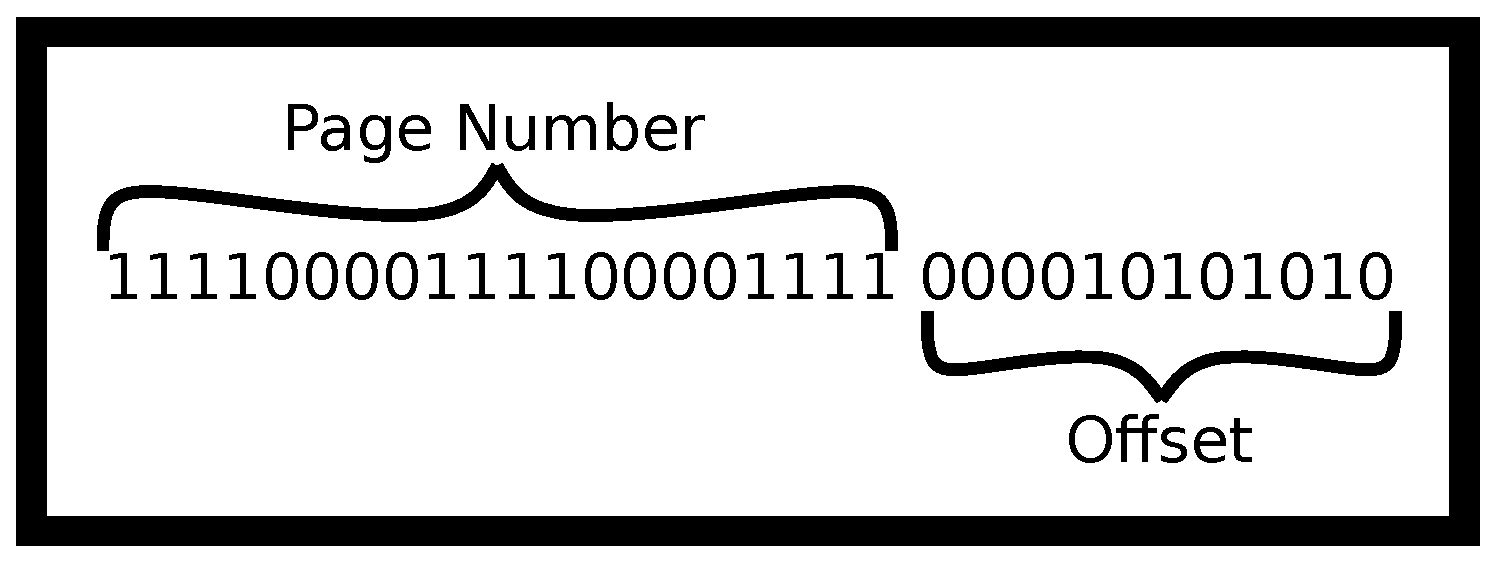
\includegraphics[width=.5\textwidth]{ipc/drawings/address_split.eps}
\caption{Splitting Address}
\end{figure}

We can imagine the steps to dereference as one process.
In general, it looks like the following.

\begin{figure}[H]
  \centering
  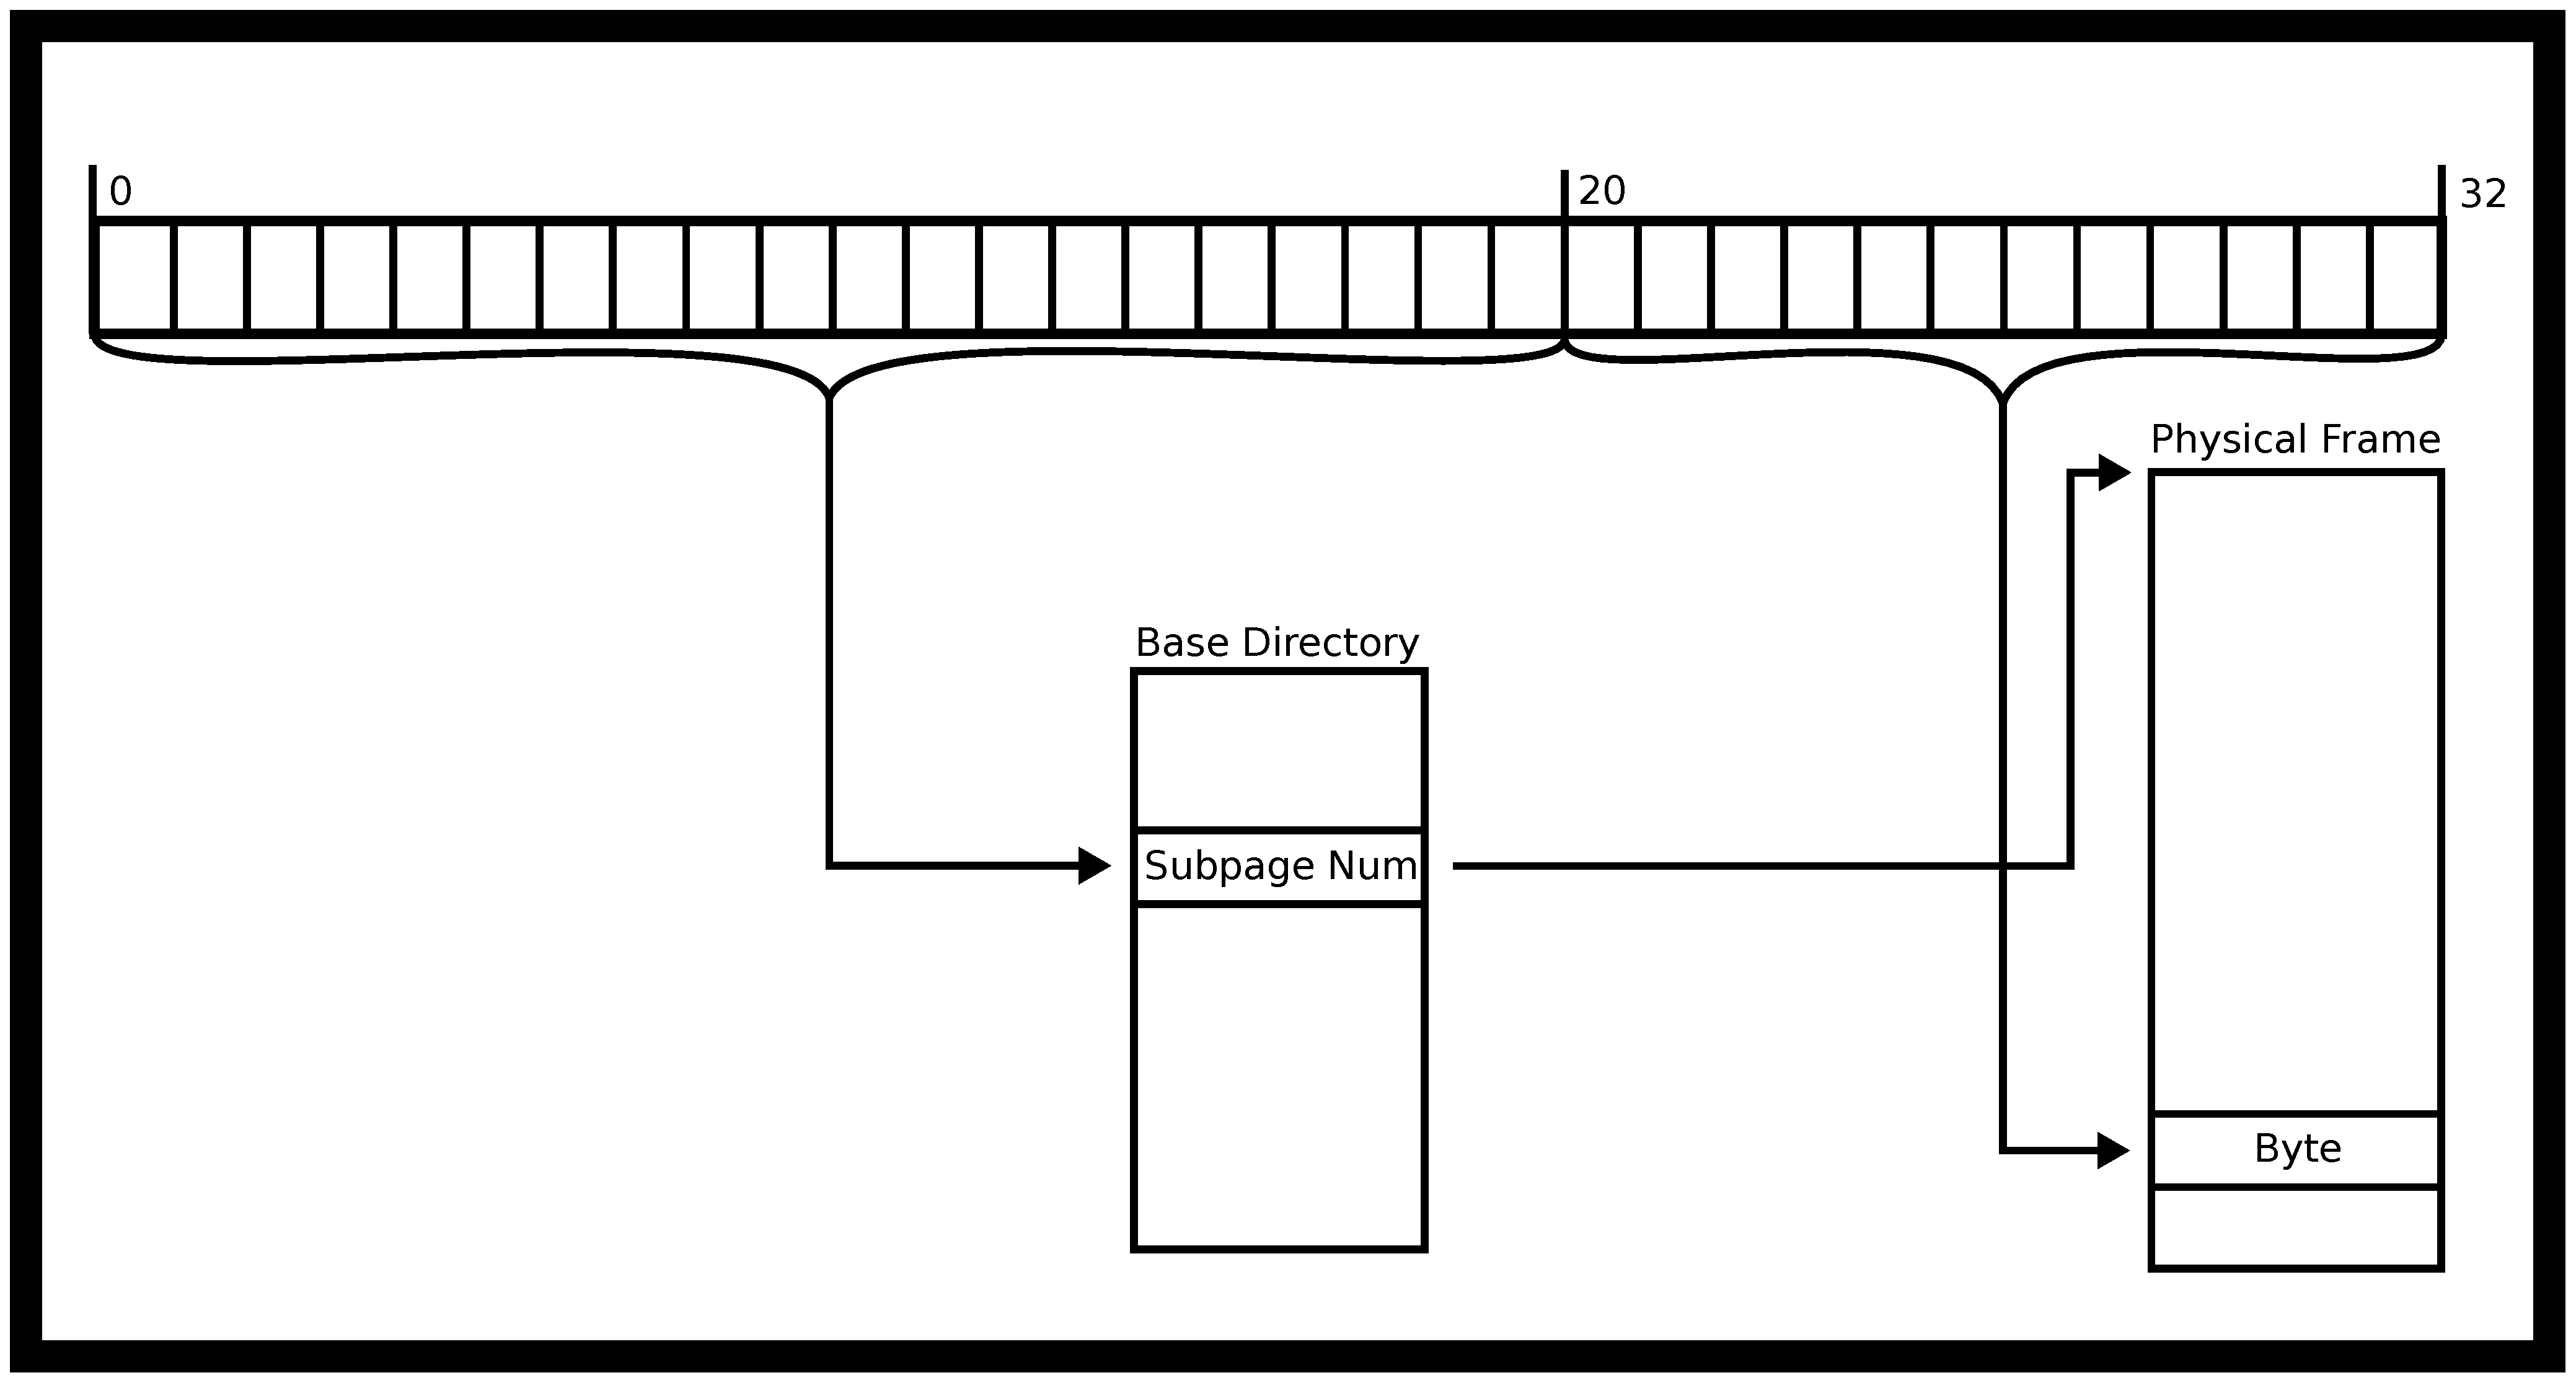
\includegraphics[width=1.0\textwidth]{ipc/drawings/level_split.eps}
  \caption{One level dereference}
\end{figure}

The way to read from a particular address above is visualized below.

\begin{figure}[H]
  \centering
  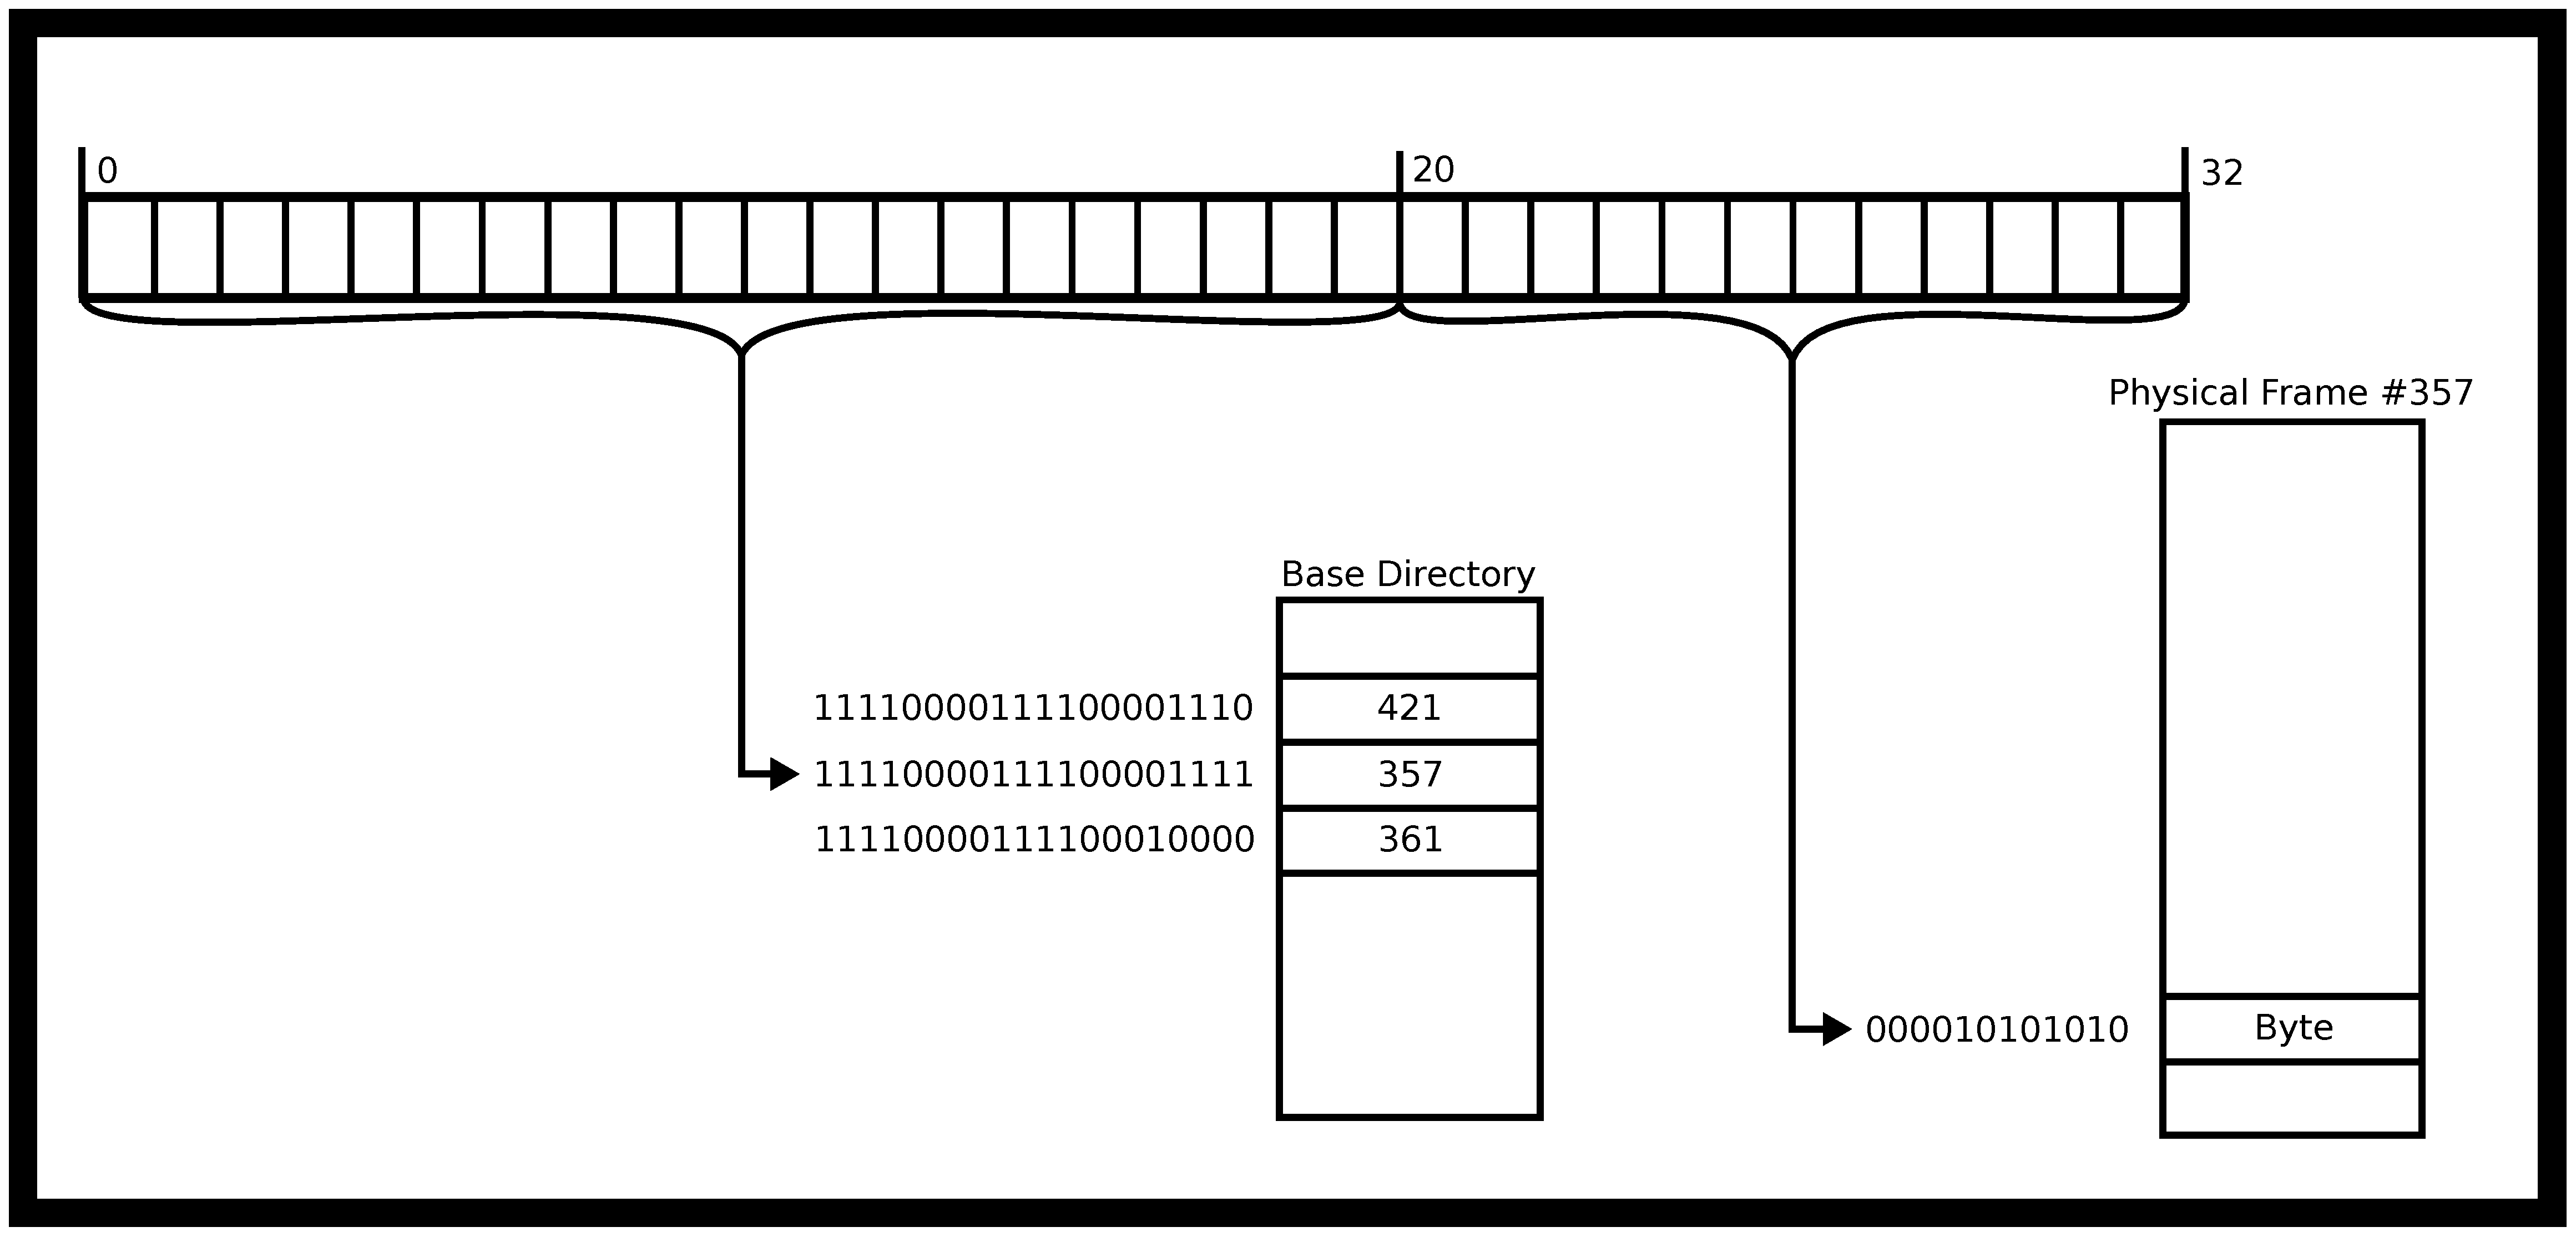
\includegraphics[width=1.0\textwidth]{ipc/drawings/level_split_filled.eps}
  \caption{One level dereference example}
\end{figure}

And if we were reading from it, 'return' that value.
This sounds like a perfect solution.
Take each address and map it to a virtual address in sequential order.
The process will believe that the address looks continuous, but the top 20 bits are used to figure out \keyword{page\_num},
which will allow us to find the frame number, find the frame, add the \textbf{offset} -- derived from the last 12 bits -- and do the read or write.

There are other ways to split it as well.
On a machine with page size 256 Bytes, then the lowest 8 bits (10101010) will be used as the offset.
The remaining upper bits will be the page number (111100001111000011110000). This offset is treated as a binary number and is added to the start of the frame when we get it.

We do have a problem with 64-bit operating systems.
For a 64-bit machine with 4KiB pages, each entry needs 52 bits.
Meaning we need roughly
With $2^{52}$ entries thats $2^{55}$ bytes (roughly 40 petabytes).
So our page table is too large.
In 64-bit architecture, memory addresses are sparse, so we need a mechanism to reduce the page table size, given that most of the entries will never be used.
We'll take about this below. There is one last piece of terminology that needs to be covered.

\subsection{Multi-level page tables}

Multi-level pages are one solution to the page table size issue for 64-bit architectures.
We'll look at the simplest implementation - a two-level page table.
Each table is a list of pointers that point to the next level of tables, not all sub-tables need to exist.
An example, two-level page table for a 32-bit architecture is shown below.

\begin{figure}[H]
\centering
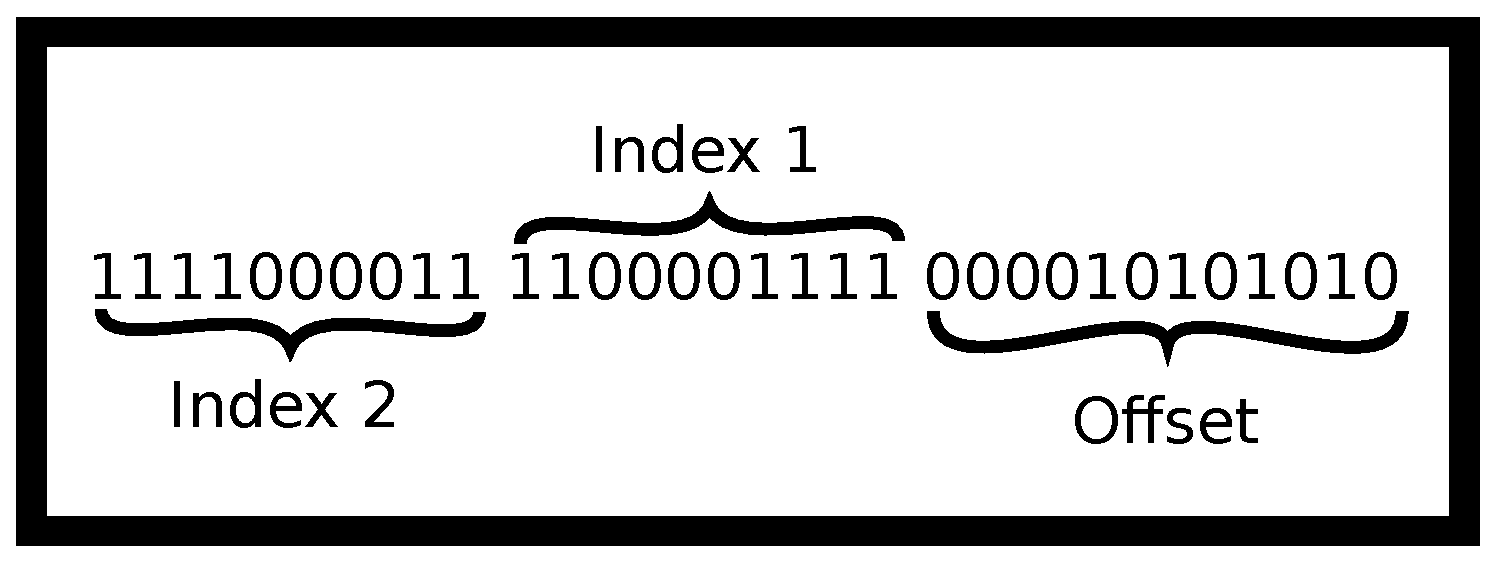
\includegraphics[width=.5\textwidth]{ipc/drawings/three_address_split.eps}
\caption{Three Way Address Split}
\end{figure}

So what is the intuition for dereferencing an address?
First, the MMU takes the top-level page table and find the \keyword{Index1}'th entry.
That will contain a number that will lead the MMU to the appropriate sub-table
Then go to the \keyword{Index2}'th entry of that table.
That will contain a frame number.
This is the good old fashioned 4KiB RAM that we were talking about earlier.
Then, the MMU adds the offset and do the read or write.

\subsubsection{Visualizing The Dereference}

In one diagram, the dereference looks like the following image.

\begin{figure}[H]
  \centering
  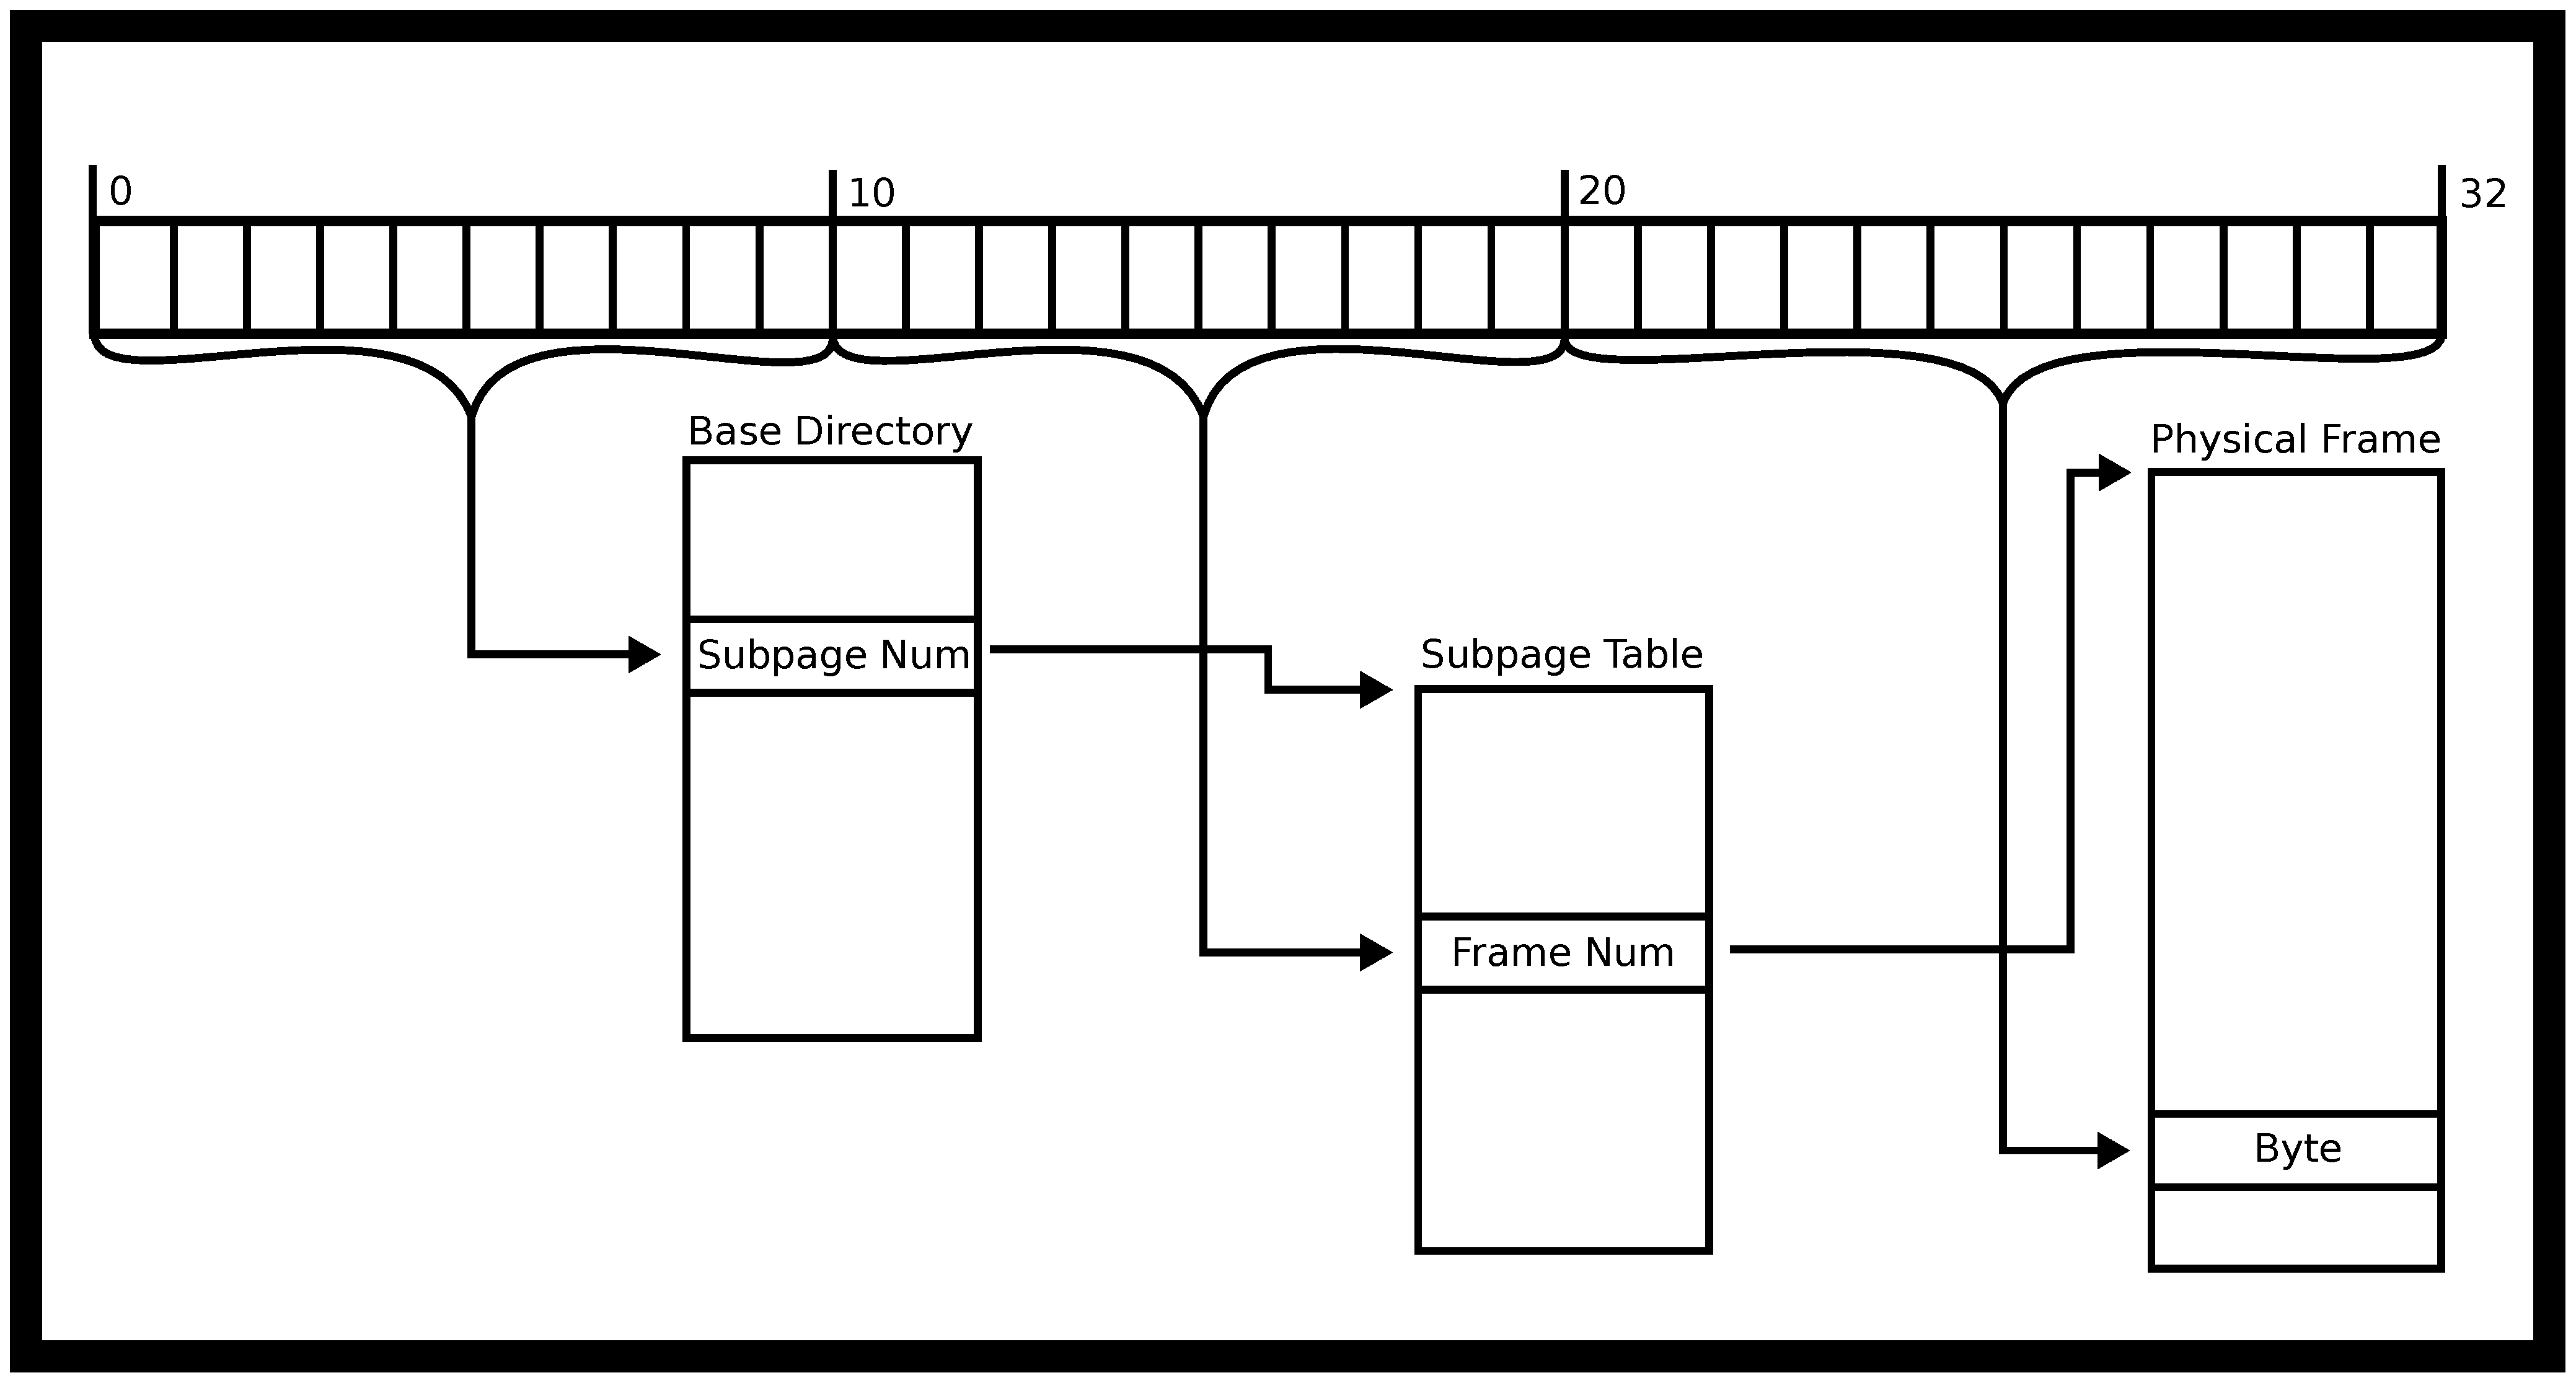
\includegraphics[width=1.0\textwidth]{ipc/drawings/multi_level_split.eps}
  \caption{Full page table dereference}
\end{figure}

Following our example, here is what the dereference would look like.

\begin{figure}[H]
  \centering
  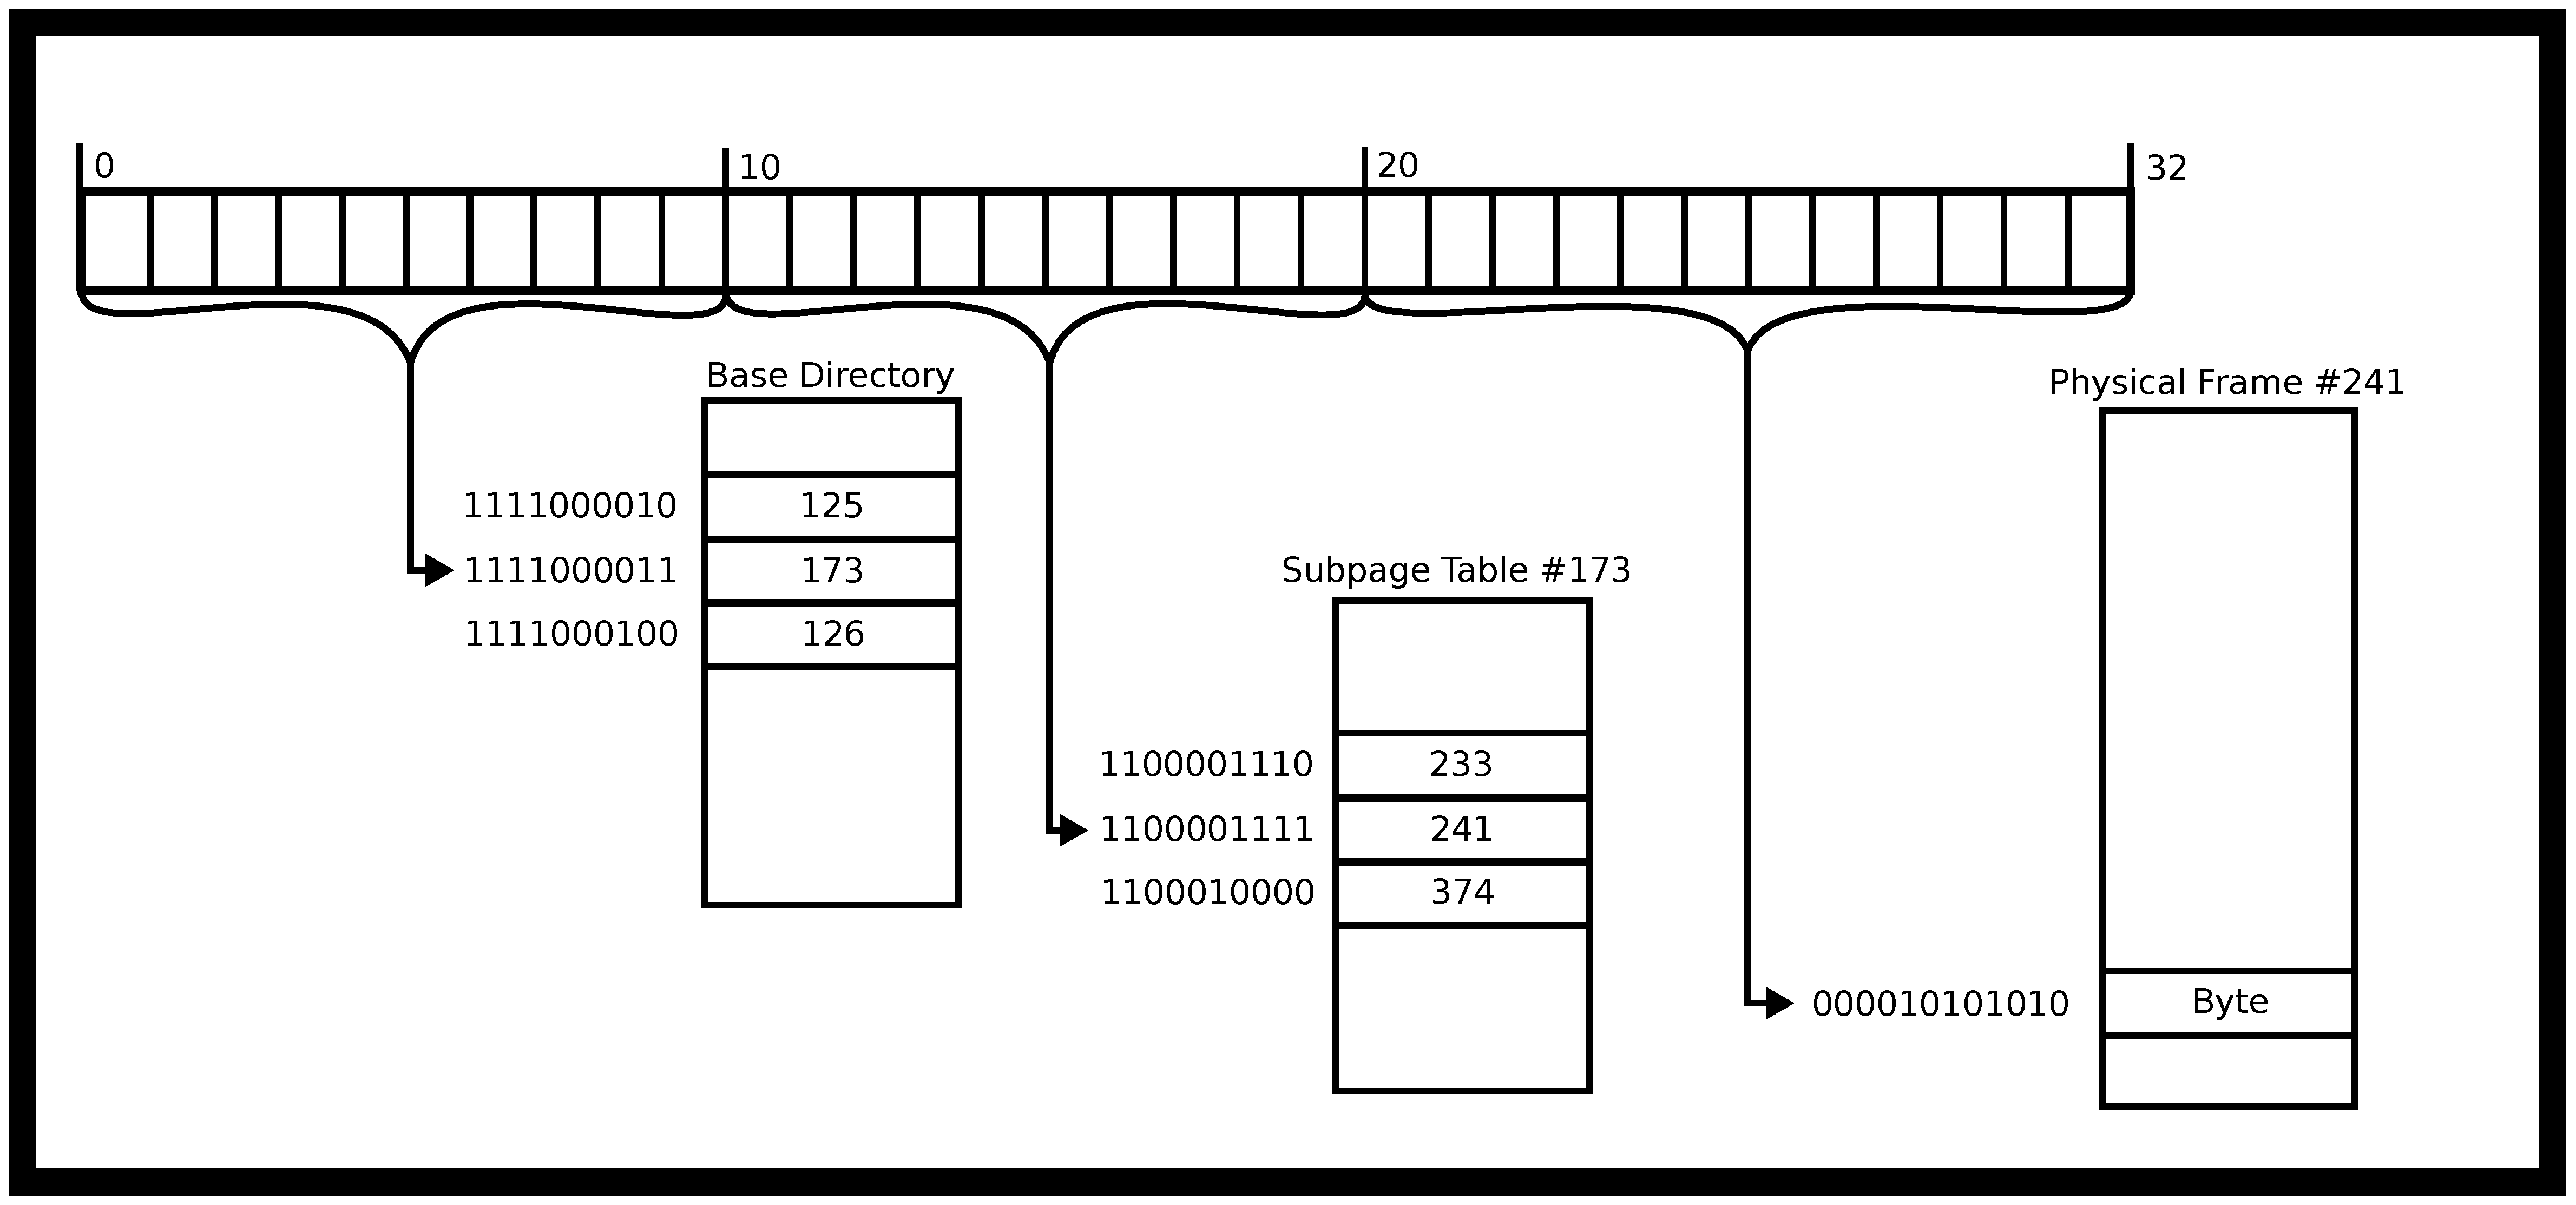
\includegraphics[width=1.0\textwidth]{ipc/drawings/multi_level_filled.eps}
  \caption{Full page example dereference}
\end{figure}

\subsubsection{Calculating Size Concerns}

Now some calculations on size.
Each \keyword{page\_table\_num} index is 10 bits wide because there are only $2^{10}$ possible \keyword{sub-tables}, so we need 10 bits to store each directory index.
We'll round up to 2 bytes for the sake of reasoning.
If 2 bytes are used for each entry in the top-level table and there are only $2^{10}$ entries, we only need 2KiB to store this entire first level page table.
Each subtable will point to physical frames, and each of their entries need to be the required 4 bytes to be able to address all the frames as mentioned earlier.
However, for processes with only tiny memory needs, we only need to specify entries for low memory addresses for the heap and program code and high memory addresses for the stack.

Thus, the total memory overhead for our multi-level page table has shrunk from 4MiB for the single-level implementation to three page tables of memory or 2KiB for the top-level and 4KiB for the two intermediate levels or 10KiB.
Here's why.
We need at least one frame for the high-level directory and two frames for just two sub-tables.
One sub-table is necessary for the low addresses -- program code, constants and possibly a tiny heap.
The other sub-table is for higher addresses used by the environment and stack.
In practice, real programs will likely need more sub-table entries, as each subtable can only reference 1024*4KiB = 4MiB of address space.
The main point still stands.
We have significantly reduced the memory overhead required to perform page table lookups.

\subsection{Page Table Disadvantages}

There are lots of problems with page tables -- one of the big problems is that they are slow.
For a single page table, our machine is now twice as slow!
Two memory accesses are required.
For a two-level page table, memory access is now three times as slow -- three memory accesses are required.

To overcome this overhead, the MMU includes an associative cache of recently-used virtual-page-to-frame lookups.
This cache is called the TLB (``translation lookaside buffer'').
Every time a virtual address needs to be translated into a physical memory location, the TLB is queried in parallel to the page table.
For most memory accesses of most programs, there is a significant chance that the TLB has cached the results.
However if a program does not have good cache coherence, the TLB will not have the result cache and now the MMU must use the much slower page table to determine the physical frame.

\subsection{MMU Algorithm}

There is a sort of pseudocode associated with the MMU.
We will assume that this is for a single-level page table.

\begin{enumerate}
\item Receive address
\item Try to translate address according to the programmed scheme
\item If the translation fails, report an invalid address
\item Otherwise,
	\begin{enumerate}
  \item If the TLB contains the physical memory, get the physical frame from the TLB and perform the read and write.
	\item If the page exists in memory, check if the process has permissions
		to perform the operation on the page meaning the process has access
		to the page, and it is reading from the page/writing to a page
		that it has permissions to do so.
		\begin{enumerate}
		\item If so then do the dereference provide the address, cache the results in the TLB
		\item Otherwise, trigger a hardware interrupt. The kernel
			will most likely send a SIGSEGV or a Segmentation Violation.
		\end{enumerate}
	\item If the page doesn't exist in memory, generate an Interrupt.
		\begin{enumerate}
		\item The kernel could realize that this page could either be not
			allocated or on disk.
      If it fits the mapping, allocate the page and try the operation again.
		\item Otherwise, this is an invalid access and the kernel will most likely send a SIGSEGV to the process.
		\end{enumerate}
	\end{enumerate}
\end{enumerate}

How would you alter this for a multi-level page table?

\subsection{Frames and Page Protections}

Frames can be shared between processes, and this is where the heart of the chapter comes into play.
We can use these tables to communicate with processes.
In addition to storing the frame number, the page table can be used to store whether a process can write or only read a particular frame.
Read-only frames can then be safely shared between multiple processes.
For example, the C-library instruction code can be shared between all processes that dynamically load the code into the process memory.
Each process can only read that memory.
Meaning that if a program try to write to a read-only page in memory, it will \keyword{SEGFAULT}.
That is why sometimes memory accesses SEGFAULT and sometimes they don't, it all depends on if your hardware says that a program can access.

Also, processes can share a page with a child process using the \keyword{mmap} system call.
\keyword{mmap} is an interesting call because instead of tying each virtual address to a physical frame, it ties it to something else. It is an important distinction that we are talking about mmap and not memory-mapped IO in general. The \keyword{mmap} system call can't reliably be used to do other memory-mapped operations like communicate with GPUs and write pixels to the screen -- this is mainly hardware dependent.

\subsubsection{Bits on Pages}

This is \textit{heavily} dependent on the chipset.
We will include some bits that have historically been popular in chipsets.

\begin{enumerate}
\item The read-only bit marks the page as read-only.
Attempts to write to the page will cause a page fault.
The page fault will then be handled by the Kernel.
Two examples of the read-only page include sharing the C standard library between multiple processes for security you wouldn't want to allow one process to modify the library and Copy-On-Write where the cost of duplicating a page can be delayed until the first write occurs.

\item The execution bit defines whether bytes in a page can be executed as CPU instructions.
Processors may will merge these bits into one and deem a page either writable or executable.
This bit is useful because it prevents stack overflow or code injection attacks when writing user data into the heap or the stack because those are not read-only and thus not executable.
Further reading: \href{http://en.wikipedia.org/wiki/NX\_bit\#Hardware\_background}{background}

\item The dirty bit allows for performance optimization.
A page on disk that is paged into physical memory then read from, and subsequently paged out again does not needs to be written back to disk, since the page hasn't changed.
However, if the page was written to after it's paged in, its dirty bit will be set, indicating that the page must be written back to the backing store.
This strategy requires that the backing store retain a copy of the page after it is paged into memory.
When a dirty bit is not used, the backing store need only be as large as the instantaneous total size of all paged-out pages at any moment.
When a dirty bit is used, at all times some pages will exist in both physical memory and the backing store.
\item There are plenty of other bits. Take a look at your favorite architecture and see what other bits are associated!
\end{enumerate}

\subsection{Page Faults}

A page fault is when a running program tries to access some virtual memory in its address space that is not mapped to physical memory.
Page faults will also occur in other situations.
There are three types of Page Faults

\begin{enumerate}
\item \textbf{Minor} If there is no mapping yet for the page, but it is a valid address.
  This could be memory asked for by \keyword{sbrk(2)} but not written to yet meaning that the operating system can wait for the first write before allocating space -- if it was read from, the operating system could short circuit the operation to read 0.
  The OS simply makes the page, loads it into memory, and moves on.

\item \textbf{Major} If the mapping to the page is not in memory but on disk.
  What this will do is swap the page into memory and swap another page out.
  If this happens frequently enough, your program is said to \emph{thrash} the MMU.

\item \textbf{Invalid} When a program tries to write to a non-writable memory address or read to a non-readable memory address.
  The MMU generates an invalid fault and the OS will usually generate a \keyword{SIGSEGV} meaning segmentation violation meaning that the program wrote outside the segment that it could write to.

\end{enumerate}

\subsection{Link Back to IPC}

What does this have to do with IPC?
Before, you knew that processes had isolation.
One, you one didn't really know how that isolation mapped.
Two, you may not know how you can break this isolation.
To break any memory level isolation you have two avenues.
One is to ask the kernel to provide some kind of interface.
The other is to ask the kernel to map two pages of memory to the same virtual memory area and handle all the synchronization yourself.

\section{mmap}

\keyword{mmap} is a trick of virtual memory of instead of mapping a page to just a frame, that frame can be backed by a file on disk, or the frame can be shared among processes.
We can use that to read from a file on disk efficiently or sync changes to the file.
One of the big optimizations is that this does not mean that the file is allocated to memory right away.
Take the following code for example.

\begin{lstlisting}[language=C]
int fd = open(...); //File is 2 Pages
char* addr = mmap(..fd..);
addr[0] = 'l';
\end{lstlisting}

The kernel sees that the program wants to mmap the file into memory, so it will reserve some space in your address space that is the length of the file.
That means when the program writes to \keyword{addr[0]} that it writes to the first byte of the file.
The kernel can actually do some optimizations too.
Instead of loading the file into memory, it may only load pages at a time because if the file is 1024 pages.
A program may only access 3 or 4 pages making loading the entire file a waste of time.
That is why page faults are so powerful.
They let the operating system take control of when a file is used.

\subsection{mmap Definitions}

\keyword{mmap} does more than just take a file and map it to memory.
It is the general interface for creating shared memory among processes.
Currently it only supports regular files and POSIX \keyword{shmem} \cite{mmap_2018}.
Naturally, you can read all about it in the reference above, which references the current working group POSIX standard.
Some other options to note in the page will follow.

The first option is that the \keyword{flags} argument of mmap can take many options.

\begin{enumerate}
\item \keyword{PROT\_READ} This means the process can read the memory. This isn't the only flag that gives the process read permission however! The underlying file descriptor in this case must be opened with read privileges.
\item \keyword{PROT\_WRITE} This means the process can write to the memory. This has to be supplied for a process to write to a mapping. If this is supplied and \keyword{PROT\_NONE} is also supplied, the latter wins and no writes can be performed. The underlying file descriptor in this case must either be opened with write privileges or a private mapping must be supplied below
\item \keyword{PROT\_EXEC} This means the process can execute this piece of memory. Although this is not stated in POSIX documents, this shouldn't be supplied with WRITE or NONE because that would make this invalid under the NX bit or not being able to execute (respectively)
\item \keyword{PROT\_NONE} This means the process can't do anything with the mapping. This could be useful if you implement guard pages in terms of security. If you surround critical data with many more pages that can't be accessed, that decreases the chance of various attacks.
\item \keyword{MAP\_SHARED} This mapping will be synchronized to the underlying file object. The file descriptor must've been opened with write permissions in this case.
\item \keyword{MAP\_PRIVATE} This mapping will only be visible to the process itself. Useful to not thrash the operating system.
\end{enumerate}

Remember that once a program is done \keyword{mmap}ping that the program must \keyword{munmap} to tell the operating system that it is no longer using the pages allocated, so the OS can write it back to disk and give back the addresses in case another mmap needs to occur.
There are accompanying calls \keyword{msync} that take a piece of mmap'ed memory and sync the changes back to the filesystem though we won't cover that in-depth.
The other parameters to mmap are described in the annotated walkthrough below.

\subsection{Annotated mmap Walkthrough}

Below is an annotated walkthrough of the example code in the man pages.
Our command line utility will take a file, offset, and length to print.
We can assume that these are initialized correctly and the offset + length is less than the length of the file.

\begin{lstlisting}[language=C]
off_t offset;
size_t length;
\end{lstlisting}

We'll assume that all system calls succeed.
First, we have to open the file and get the size.

\begin{lstlisting}[language=C]
struct stat sb;
int fd = open(argv[1], O_RDONLY);
fstat(fd, &sb);
\end{lstlisting}

Then, we need to introduce another variable known as \keyword{page\_offset}.
mmap doesn't let the program pass in any value as an offset, it needs to be a multiple of the page size.
In our case, we will round down.

\begin{lstlisting}[language=C]
off_t page_offset = offset & ~(sysconf(_SC_PAGE_SIZE) - 1);
\end{lstlisting}

Then, we make the call to mmap, here is the order of arguments.
\begin{enumerate}
\item NULL, this tells mmap we don't need any particular address to start from
\item length + offset - page\_offset, mmaps the ``rest'' of the file into memory (starting from offset)
\item PROT\_READ, we want to read the file
\item MAP\_PRIVATE, tell the OS, we don't want to share our mapping
\item fd, object descriptor that we refer to
\item pa\_offset, the page aligned offset to start from
\end{enumerate}

\begin{lstlisting}[language=C]
char * addr = mmap(NULL, length + offset - page_offset, PROT_READ,
  MAP_PRIVATE, fd, page_offset);
\end{lstlisting}

Now, we can interact with the address as if it were a normal buffer.
After, we have to unmap the file and close the file descriptor to make sure other system resources are freed.

\begin{lstlisting}[language=C]
write(1, addr + offset - page_offset, length);
munmap(addr, length + offset - pa_offset);
close(fd);
\end{lstlisting}

Check out the full listing in the man pages.

\subsection{MMAP Communication}

So how would we use mmap to communicate across processes?
Conceptually, it would be the same as using threading.
Let's go through a broken down example.
First, we need to allocate some space.
We can do that with the \keyword{mmap} call.
We'll also allocate space for 100 integers

\begin{lstlisting}[language=C]
int size = 100 * sizeof(int);
void *addr = mmap(0, size, PROT_READ | PROT_WRITE, MAP_SHARED | MAP_ANONYMOUS, -1, 0);
int *shared = addr;
\end{lstlisting}

Then, we need to fork and perform some communication.
Our parent will store some values, and our child will read those values.

\begin{lstlisting}[language=C]
pid_t mychild = fork();
if (mychild > 0) {
  shared[0] = 10;
  shared[1] = 20;
} else {
  sleep(1); // Check the synchronization chapter for a better way
  printf("%d\n", shared[1] + shared[0]);
}
\end{lstlisting}

Now, there is no assurance that the values will be communicated because the process used \keyword{sleep} not a mutex.
Most of the time this will work.

\begin{lstlisting}[language=C]
#include <stdio.h>
#include <stdlib.h>
#include <sys/types.h>
#include <sys/stat.h>
#include <sys/mman.h> /* mmap() is defined in this header */
#include <fcntl.h>
#include <unistd.h>
#include <errno.h>
#include <string.h>

int main() {

  int size = 100 * sizeof(int);
  void *addr = mmap(0, size, PROT_READ | PROT_WRITE, MAP_SHARED | MAP_ANONYMOUS, -1, 0);

  printf("Mapped at %p\n", addr);

  int *shared = addr;
  pid_t mychild = fork();
  if (mychild > 0) {
    shared[0] = 10;
    shared[1] = 20;
  } else {
    sleep(1); // We will talk about synchronization later
    printf("%d\n", shared[1] + shared[0]);
  }

  munmap(addr,size);
  return 0;
}
\end{lstlisting}

This piece of code allocates space for a 100 integers and creates a piece of memory that is shared between all processes.
The code then forks.
The parent process writes two integers to the first two slots.
To avoid a data race, the child sleeps for a second and then prints out the stored values.
This is not a perfect way to protect against data races.
We could use a mutex across processes mentioned in the synchronization section.
But for this simple example, it works just fine.
Note that each process should call munmap when done using the piece of memory.

Sharing anonymous memory is a very efficient form of inter-process communication because there is no copying, system call, or disk-access overhead - the two processes literally share the same physical frame of main memory.
On the other hand, shared memory, like in a multithreading context, creates room for data races.
Processes that share writable memory might need to use synchronization primitives like mutexes to prevent these from happening.

\section{Pipes}

You've seen the virtual memory way of IPC, but there are more standard versions of IPC that are provided by the kernel.
One of the big utilities is POSIX pipes.
A pipe simply takes in a stream of bytes and spits out a sequence of bytes.

One of the big starting points of pipes was way back in the PDP-10 days. In those days, a write to the disk or even your terminal was very slow as it may have to be printed out.
The Unix programmers still wanted to create small, portable programs that did one thing very well and could be composed.
As such, pipes were invented to take the output of one program
and feed it to the input of another program though they have other uses today -- you can read more \href{https://en.wikipedia.org/wiki/Pipeline\_\%28Unix\%29}{At the wikipedia page}
Consider if you type the following into your terminal.

\begin{lstlisting}[language=bash]
$ ls -1 | cut -d'.' -f1 | sort | uniq | tee dirents
\end{lstlisting}

What does the following code do?
First, it lists the current directory.
The -1 means that it outputs one entry per line.
The \keyword{cut} command then takes everything before the first period.
\keyword{sort} sorts all the input lines, \keyword{uniq} makes sure all the lines are uniq.
Finally, \keyword{tee} outputs the contents to the file \keyword{dir\_contents} and the terminal for your perusal.
The important part is that bash creates \textbf{5 separate processes} and connects their standard outs/stdins with pipes the trail looks something like this.

\begin{figure}[H]
  \centering
  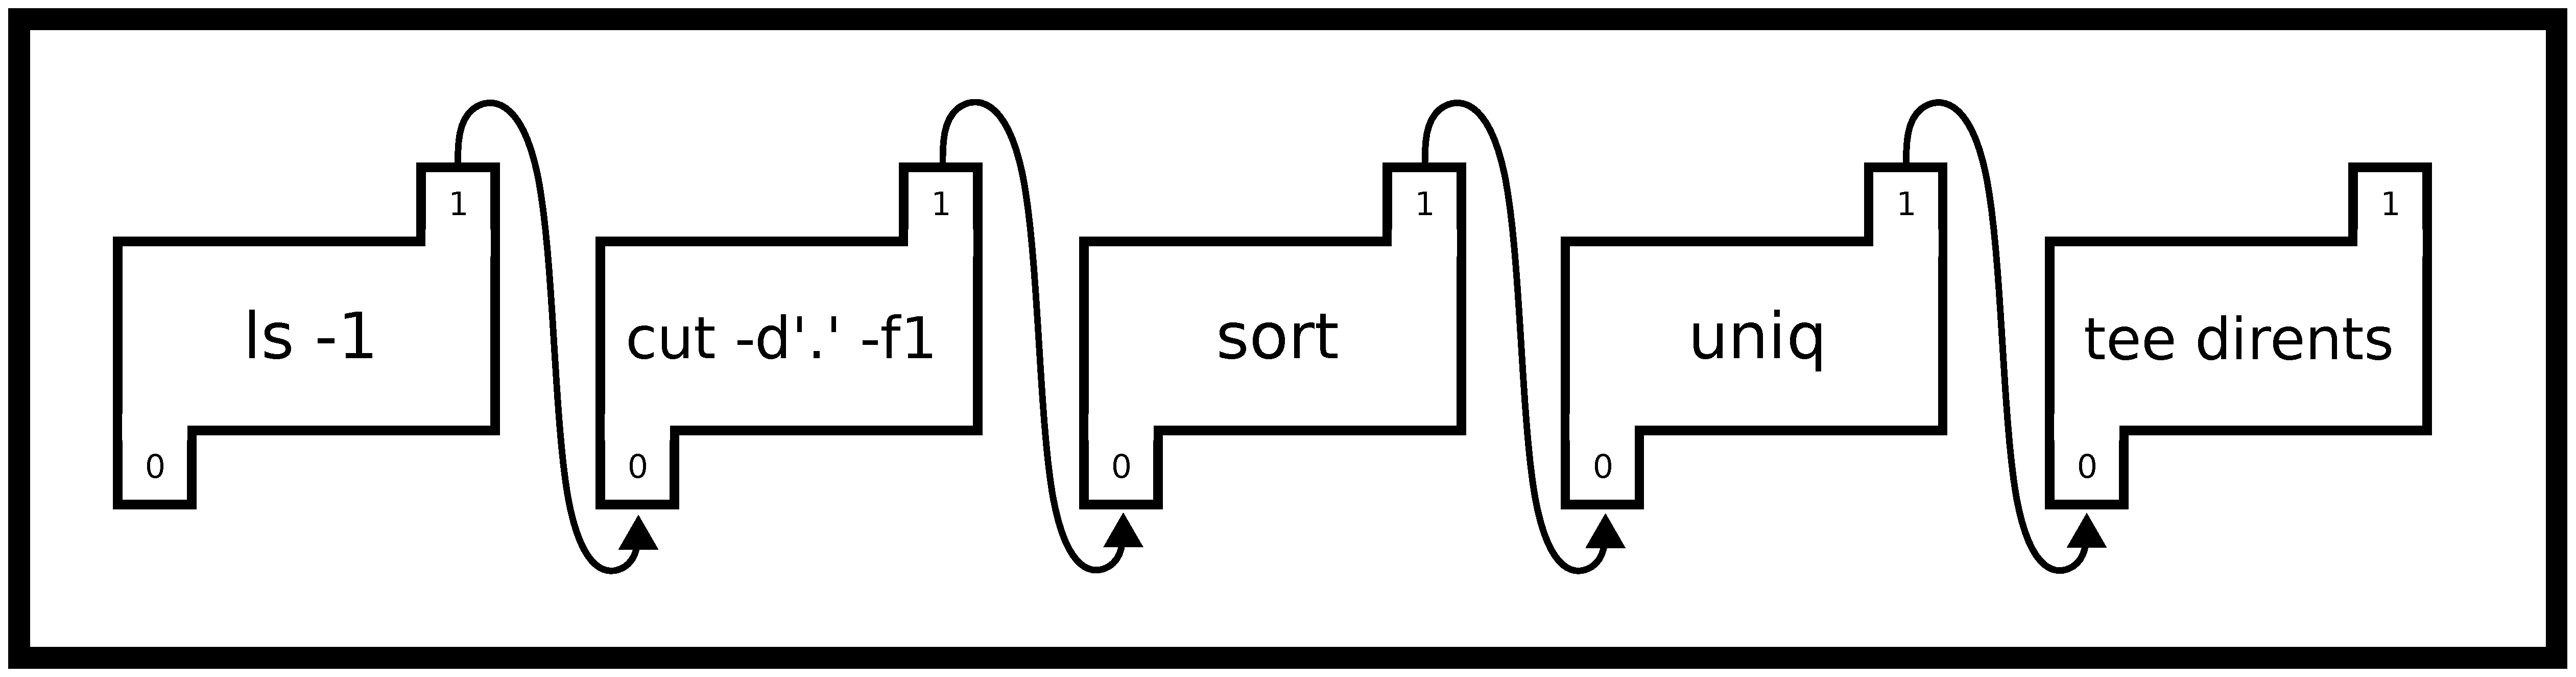
\includegraphics[width=.8\textwidth]{ipc/drawings/pipe_process.eps}
  \caption{Pipe Process Filedescriptor redirection}
\end{figure}

The numbers in the pipes are the file descriptors for each process and the arrow represents the redirect or where the output of the pipe is going.
A POSIX pipe is almost like its real counterpart - a program can stuff bytes down one end and they will appear at the other end in the same order.
Unlike real pipes, however, the flow is always in the same direction, one file descriptor is used for reading and the other for writing.
The \keyword{pipe} system call is used to create a pipe.
These file descriptors can be used with \keyword{read} and \keyword{write}.
A common method of using pipes is to create the pipe before forking to communicate with a child process

\begin{lstlisting}[language=C]
int filedes[2];
pipe (filedes);
pid_t child = fork();
if (child > 0) { /* I must be the parent */
  char buffer[80];
  int bytesread = read(filedes[0], buffer, sizeof(buffer));
  // do something with the bytes read
} else {
  write(filedes[1], "done", 4);
}
\end{lstlisting}

There are two file descriptors that pipe creates.
\keyword{filedes[0]} contains the read end.
\keyword{filedes[1]} contains the write end.
How your friendly neighborhood TAs remember it is one can \textit{read before they can write, or reading comes before writing}.
You can groan all you want at it, but it is helpful to remember what is the read end and what is the write end.

One can use pipes inside of the same process, but there tends to be no added benefit.
Here's an example program that sends a message to itself.

\begin{lstlisting}[language=C]
#include <unistd.h>
#include <stdlib.h>
#include <stdio.h>

int main() {
  int fh[2];
  pipe(fh);
  FILE *reader = fdopen(fh[0], "r");
  FILE *writer = fdopen(fh[1], "w");
  // Hurrah now I can use printf
  printf("Writing...\n");
  fprintf(writer,"%d %d %d\n", 10, 20, 30);
  fflush(writer);

  printf("Reading...\n");
  int results[3];
  int ok = fscanf(reader,"%d %d %d", results, results + 1, results + 2);
  printf("%d values parsed: %d %d %d\n", ok, results[0], results[1], results[2]);

  return 0;
}
\end{lstlisting}

The problem with using a pipe in this fashion is that writing to a pipe can block meaning the pipe only has a limited buffering capacity.
The maximum size of the buffer is system-dependent; typical values from 4KiB up to 128KiB though they can be changed.

\begin{lstlisting}[language=C]
int main() {
  int fh[2];
  pipe(fh);
  int b = 0;
  #define MESG "..............................."
  while(1) {
    printf("%d\n",b);
    write(fh[1], MESG, sizeof(MESG))
    b+=sizeof(MESG);
  }
  return 0;
}
\end{lstlisting}

\subsection{Pipe Gotchas}

Here's a complete example that doesn't work!
The child reads one byte at a time from the pipe and prints it out - but we never see the message!
Can you see why?

\begin{lstlisting}[language=C]
#include <stdio.h>
#include <stdlib.h>
#include <unistd.h>
#include <signal.h>

int main() {
  int fd[2];
  pipe(fd);
  //You must read from fd[0] and write from fd[1]
  printf("Reading from %d, writing to %d\n", fd[0], fd[1]);

  pid_t p = fork();
  if (p > 0) {
    /* I have a child, therefore I am the parent */
    write(fd[1],"Hi Child!",9);

    /*don't forget your child*/
    wait(NULL);
  } else {
    char buf;
    int bytesread;
    // read one byte at a time.
    while ((bytesread = read(fd[0], &buf, 1)) > 0) {
      putchar(buf);
    }
  }
  return 0;
}
\end{lstlisting}

The parent sends the bytes \keyword{H,i,(space),C...!} into the pipe.
The child starts reading the pipe one byte at a time.
In the above case, the child process will read and print each character.
However, it never leaves the while loop!
When there are no characters left to read it simply blocks and waits for more unless \textbf{All the writers close their ends}
Another solution could also exit the loop by checking for an end-of-message marker,

\begin{lstlisting}[language=C]
while ((bytesread = read(fd[0], &buf, 1)) > 0) {
  putchar(buf);
  if (buf == '!') break; /* End of message */
}
\end{lstlisting}

We know that when a process tries to read from a pipe where there are still writers, the process blocks.
If no pipe has no writers, read returns 0.
If a process tries to write with some reader's read goes through, or fails -- partially or completely -- if the pipe is full.
Why happens when a process tries to write when there are no readers left?

\begin{verbatim}
If all file descriptors referring to the read end of a pipe have been closed,
then a write(2) will cause a SIGPIPE signal to be generated for the calling process.
\end{verbatim}

Tip: Notice only the writer (not a reader) can use this signal.
To inform the reader that a writer is closing their end of the pipe, a program could write your own special byte (e.g.~0xff) or a message (\keyword{"Bye!"})

Here's an example of catching this signal that does not work! Can you see why?

\begin{lstlisting}[language=C]
#include <stdio.h>
#include <stdio.h>
#include <unistd.h>
#include <signal.h>

void no_one_listening(int signal) {
  write(1, "No one is listening!\n", 21);
}

int main() {
  signal(SIGPIPE, no_one_listening);
  int filedes[2];

  pipe(filedes);
  pid_t child = fork();
  if (child > 0) {
    /* This process is the parent. Close the listening end of the pipe */
    close(filedes[0]);
  } else {
    /* Child writes messages to the pipe */
    write(filedes[1], "One", 3);
    sleep(2);
    // Will this write generate SIGPIPE ?
    write(filedes[1], "Two", 3);
    write(1, "Done\n", 5);
  }
  return 0;
}
\end{lstlisting}

The mistake in the above code is that there is still a reader for the pipe!
The child still has the pipe's first file descriptor open and remember the specification? All readers must be closed

When forking, \emph{It is common practice} to close the unnecessary (unused) end of each pipe in the child and parent process.
For example, the parent might close the reading end and the child might close the writing end.

The last addendum is that a program can set the file descriptor to return when there is no one listening instead of SIGPIPE because by default SIGPIPE terminates your program.
The reason that this is default behavior is it makes the pipe example above work.
Consider this useless use of cat

\begin{lstlisting}[language=bash]
$ cat /dev/urandom | head -n 20
\end{lstlisting}
Which grabs 20 lines of input from urandom. \keyword{head} will terminate after 20 newline characters have been read.
What about \keyword{cat}?
\keyword{cat} needs to receive a SIGPIPE informing it that the program just tried to write to a pipe that no one is listening on.

\subsection{Other pipe facts}

A pipe gets filled up when the writer writes too much to the pipe without the reader reading any of it. When the pipes become full, all writes fail until a read occurs. Even then, a write may partial fail if the pipe has a little bit of space left but not enough for the entire message. Usually, two things are done to avoid this. Either increase the size of the pipe. Or more commonly, fix your program design so that the pipe is constantly being read from.

As hinted at before, Pipe writes are atomic up to the size of the pipe. Meaning that if two processes try to write to the same pipe, the kernel has internal mutexes with the pipe that it will lock, do the write, and return. The only gotcha is when the pipe is about to become full. If two processes are trying to write and the pipe can only satisfy a partial write, that pipe write is not atomic -- be careful about that!

Unnamed pipes live in memory and are a simple and efficient form of inter-process communication (IPC) that is useful for streaming data and simple messages. Once all processes have closed, the pipe resources are freed.

It is also common design for a pipe to be one way -- meaning one process should do the writing and one process do the reading. Otherwise, the child would attempt to read its own data intended for the parent (and vice versa)!

\subsection{Pipes and Dup}

Often, you'll want to use \keyword{pipe2} in combination with dup.
Take for example the simple program in the command line.

\begin{lstlisting}[language=bash]
$ ls -1 | cut -f1 -d.
\end{lstlisting}

This command takes the output of \keyword{ls -1} which lists the content of the current directory on one line each and pipes it to cut.
Cut take a delimiter, in this case a dot, and a field position, in our case 1, and outputs per line the nth field by each delimiter.
At a high level, this grabs the file names without the extension of our current directory.

Underneath the hood, this is how bash does it internally.

\begin{lstlisting}[language=C]
#define _GNU_SOURCE

#include <stdio.h>
#include <fcntl.h>
#include <unistd.h>
#include <stdlib.h>

int main() {

  int pipe_fds[2];
  // Call with the O_CLOEXEC flag to prevent any commands from blocking
  pipe2(pipe_fds, O_CLOEXEC);

  // Remember for pipe_fds, the program read then write (reading is 0 and writing is 1)

  if(!fork()) {
    // Child

    // Make the stdout of the process, the write end
    dup2(pipe_fds[1], 1);

    // Exec! Don't forget the cast
    execlp("ls", "ls", "-1", (char*)NULL);
    exit(-1);
  }

  // Same here, except the stdin of the process is the read end
  dup2(pipe_fds[0], 0);

  // Same deal here
  execlp("cut", "cut", "-f1", "-d.", (char*)NULL);
  exit(-1);

  return 0;
}
\end{lstlisting}

The results of the two programs should be the same.
Remember as you encounter more complicated examples of piping processes up, a program needs to close all unused ends of pipes otherwise the program will deadlock waiting for your processes to finish.

\subsection{Pipe Conveniences}

If the program already have a file descriptor, it can `wrap' it yourself into a FILE pointer using \keyword{fdopen}.

\begin{lstlisting}[language=C]
#include <sys/types.h>
#include <sys/stat.h>
#include <fcntl.h>

int main() {
  char *name="Fred";
  int score = 123;
  int filedes = open("mydata.txt", "w", O_CREAT, S_IWUSR | S_IRUSR);

  FILE *f = fdopen(filedes, "w");
  fprintf(f, "Name:%s Score:%d\n", name, score);
  fclose(f);
\end{lstlisting}

For writing to files this is unnecessary - just use \keyword{fopen} which does the same as \keyword{open} and \keyword{fdopen} However for pipes, we already have a file descriptor - so this is a great time to use \keyword{fdopen}

Here's a complete example using pipes that almost works!
Can you spot the error?
Hint: The parent never prints anything!

\begin{lstlisting}[language=C]
#include <unistd.h>
#include <stdlib.h>
#include <stdio.h>

int main() {
  int fh[2];
  pipe(fh);
  FILE *reader = fdopen(fh[0], "r");
  FILE *writer = fdopen(fh[1], "w");
  pid_t p = fork();
  if (p > 0) {
    int score;
    fscanf(reader, "Score %d", &score);
    printf("The child says the score is %d\n", score);
  } else {
    fprintf(writer, "Score %d", 10 + 10);
    fflush(writer);
  }
  return 0;
}
\end{lstlisting}

Note the unnamed pipe resource will disappear once both the child and parent have exited.
In the above example, the child will send the bytes and the parent will receive the bytes from the pipe.
However, no end-of-line character is ever sent, so \keyword{fscanf} will continue to ask for bytes because it is waiting for the end of the line i.e.~it will wait forever! The fix is to ensure we send a newline character so that \keyword{fscanf} will return.

\begin{lstlisting}[language=C]
change:   fprintf(writer, "Score %d", 10 + 10);
to:       fprintf(writer, "Score %d\n", 10 + 10);
\end{lstlisting}

If you want your bytes to be sent to the pipe immediately, you'll need to fflush!
Remember back to the introduction section that shows the difference between terminal vs non-terminal outputs of stdout.

\textbf{Even though we have a section on it, it is highly not recommended to fdopen() anything that doesn't point to an underlying file descriptors}.
The reason being is that while we get conveniences we also get annoyances like the buffering example we mentioned, caching, etc.
The basic C library motto is that any device a program can properly \keyword{fseek} or move to an arbitrary position, it should be able to \keyword{fdopen}.
Files satisfy this behavior, shared memory also, terminals, etc.
When it comes to pipes, sockets, epoll objects, etc, don't do it.

\section{Named Pipes}

An alternative to \emph{unnamed} pipes is \emph{named} pipes created using \keyword{mkfifo}.
From the command line: \keyword{mkfifo} From C: \keyword{int\ mkfifo(const\ char\ *pathname,\ mode\_t\ mode);}

You give it the pathname and the operation mode, it will be ready to go!
Named pipes take up virtually no space on disk.
This means the actual contents of the pipe aren't printed to the file and read from that same file.
What the operating system tells you when you have a named pipe is that it will create an unnamed pipe that refers to the named pipe, and that's it!
There is no additional magic.
This is just for programming convenience if processes are started without forking meaning that there would be no way to get the file descriptor to the child process for an unnamed pipe.

\subsection{Why is my named pipe hanging?}

A named pipe \keyword{mkfifo} is a pipe that a program calls \keyword{open(2)} on with read and/or write permissions.
This is useful if you want to have a pipe between two processes without one processing having to fork the other process.
There are some gotchas with named pipes.
There is more down below, but we'll introduce it here for a simple example.
Reads and writes hang on Named Pipes until there is at least one reader and one writer, take this.

\begin{lstlisting}[language=bash]
1$ mkfifo fifo
1$ echo Hello > fifo
# This will hang until the following command is run on another terminal or another process
2$ cat fifo
Hello
\end{lstlisting}

Any \keyword{open} is called on a named pipe the kernel blocks until another process calls the opposite open. Meaning, echo calls \keyword{open(..,\ O\_RDONLY)} but that blocks until cat calls \keyword{open(..,\ O\_WRONLY)}, then the programs are allowed to continue.

\subsection{Race condition with named pipes}

What is wrong with the following program?

\begin{lstlisting}[language=C]
//Program 1

int main(){
  int fd = open("fifo", O_RDWR | O_TRUNC);
  write(fd, "Hello!", 6);
  close(fd);
  return 0;
}

//Program 2
int main() {
  char buffer[7];
  int fd = open("fifo", O_RDONLY);
  read(fd, buffer, 6);
  buffer[6] = '\0';
  printf("%s\n", buffer);
  return 0;
}
\end{lstlisting}

This may never print hello because of a race condition.
Since a program opened the pipe in the first process under both permissions, open won't wait for a reader because the program told the operating system that it is a reader!
Sometimes it looks like it works because the execution of the code looks something like this.

\begin{tabular}{|c|c|c|}
  & Process 1 & Process 2 \\ \hline
  Time 1 & open(O\_RDWR) \& write() & \\
  Time 2 & & open(O\_RDONLY) \& read() \\
  Time 3 & close() \& exit() & \\
  Time 4 & print() \& exit() & \\
\end{tabular}

But here is an invalid series of operations that cause a race condition.

\begin{tabular}{|c|c|c|}
  & Process 1 & Process 2 \\ \hline
  Time 1 & open(O\_RDWR) \& write() & \\
  Time 2 & close() \& exit() & \\
  Time 3 & & open(O\_RDONLY) (Blocks Indefinitely) \\
\end{tabular}

\section{Files}

On Linux, there are two abstractions with files. The first is the Linux \keyword{fd} level abstraction.

 \begin{itemize}
\item \keyword{open} takes a path to a file and creates a file descriptor entry in the process table. If the file is not available, it errors out.
\item \keyword{read} takes a number of bytes that the kernel has received and reads them into a user space buffer. If the file is not open in read mode, this will break.
\item \keyword{write} outputs a number of bytes to a file descriptor. If the file is not open in write mode, this will break. This may be buffered internally.
\item \keyword{close} removes a file descriptor from a process' file descriptors. This always succeeds on a valid file descriptor.
\item \keyword{lseek} takes a file descriptor and moves it to a certain position. Can fail if the seek is out of bounds.
\item \keyword{fcntl} is the catch-all function for file descriptors. Set file locks, read, write, edit permissions, etc \ldots{}
 \end{itemize}

The Linux interface is very powerful and expressive, but sometimes we need portability for example if we are writing for a Macintosh or windows.
This is where C's abstraction comes into play.
On different operating systems, C uses the low-level functions to create a wrapper around files used everywhere, meaning that C on Linux uses the above calls.

\begin{itemize}
\item \keyword{fopen} opens a file and returns an object. \keyword{null} is returned if the program doesn't have permission for the file.
\item \keyword{fread} reads a certain number of bytes from a file. An error is returned if already at the end of the file when which the program must call \keyword{feof()} to check if the program attempted to read \textit{past} the end of the file.
\item \keyword{fgetc/fgets} Get a char or a string from a file
\item \keyword{fscanf} Read a format string from the file
\item \keyword{fwrite} Write some objects to a file
\item \keyword{fprintf} Write a formatted string to a file
\item \keyword{fclose} Close a file handle
\item \keyword{fflush} Take any buffered changes and flush them to a file
\end{itemize}

But programs don't get the expressiveness that Linux gives with system calls.
A program can convert back and forth between them with \keyword{int\ fileno(FILE*\ stream)} and \keyword{FILE*\ fdopen(int\ fd...)}.
Also, C files are \textbf{buffered} meaning that their contents may not be written right away by default.
You can change that with C options.

\textbf{Danger} With portability you lose something important, the ability to tell an error.
A program can \keyword{fopen} a file descriptor and get a \keyword{FILE*} object but \textbf{it won't be the same as a file} meaning that certain calls will fail or act weirdly.
The C API reduces this weirdness, but for example a program cannot \keyword{fseek} to a part of the file, or perform any operations with its buffering.
The problem is the API won't give a lot of warning because C needs to maintain compatibility with other operating systems.
To keep things simple, use the C API of files when dealing with a file on disk, which will work fine. Otherwise, be in for a rough ride for portability sake.

\subsection{Determining File Length}

For files less than the size of a long, using fseek and ftell is a
simple way to accomplish this.
Move to the end of the file and find out the current position.

\begin{lstlisting}[language=C]
fseek(f, 0, SEEK_END);
long pos = ftell(f);
\end{lstlisting}

This tells us the current position in the file in bytes - i.e.~the
length of the file!

\keyword{fseek} can also be used to set the absolute position.

\begin{lstlisting}[language=C]
fseek(f, 0, SEEK_SET); // Move to the start of the file
fseek(f, posn, SEEK_SET);  // Move to 'posn' in the file.
\end{lstlisting}

All future reads and writes in the parent or child processes will honor this position.
Note writing or reading from the file will change the current position.
See the man pages for fseek and ftell for more information.

\subsection{But don't do this}

\textbf{Note: This is not recommended in the usual case because of a quirk with the C language}.
That quirk is that longs only need to be \textbf{4 Bytes big} meaning that the maximum size that \keyword{ftell} can return is a little under 2 Gibibytes which we know nowadays our files could be hundreds of gibibytes or even terabytes on a distributed file system.
What should we do instead? Use \keyword{stat}! We will cover stat in a later part but here is some code that will tell a program the size of the file

\begin{lstlisting}[language=C]
struct stat buf;
if(stat(filename, &buf) == -1){
  return -1;
}
return (ssize_t)buf.st_size;
\end{lstlisting}

\keyword{buf.st\_size} is of type \keyword{off\_t} which is big enough for large files.

\subsection{Gotchas with files}

What happens when file streams are closed by two different processes?
Closing a file stream is unique to each process.
Other processes can continue to use their own file-handle.
Remember, everything is copied over when a child is created, even the relative positions of the files.
As you might have observed with using \keyword{fork}, there is a quirk of the implementation of files and their caches on Ubuntu that will rewind a file descriptor once a file has been closed.
As such, make sure to close before forking or at least don't trigger a cache inconsistency which is much harder.

\section{IPC Alternativs}

Okay so now you have a list of tools in your toolbox to tackle communicating between processes, so what should you use?

There really is no hard answer, though this is the most interesting question.
Generally, we have retained pipes for legacy reasons.
This means that we only really use them to redirect stdin, stdout, and stderr for the collection of logs and similar programs.
You may find processes trying to communicate with unnamed or named pipes as well.
Most of the time you won't be dealing with this interaction directly though.

Files are used almost all the time as a form of IPC.
Hadoop is a great example where processes will write to append-only tables and then other processes will read from those tables.
We generally use files under a few cases.
One case is if we want to save the intermediate results of an operation to a file for future use.
Another case is if putting it in memory would cause an out of memory error.
On Linux, file operations are generally pretty cheap, so most programmers use it as larger intermediate storage.

mmap is used for two scenarios.
One is a \keyword{linear} or \keyword{near-linear} read through of the file.
Meaning, a program reads the file front to back or back to front.
The key is that the program don't jump around too much.
Jumping around too much causes thrashing and loses all the benefits of using mmap.
The other case of mmap is a direct memory inter-process communication.
This means that a program can store structures in a piece of mmap'ed memory and share them between two processes.
Python and Ruby use this mapping all the time to utilize copy on write semantics.

\section{Topics}

\begin{enumerate}
  \item Virtual Memory
  \item Page Table
  \item MMU/TLB
  \item Address Translation
  \item Page Faults
  \item Frames/Pages
  \item Single-level vs multi-level page table
  \item Calculating offsets for multi-level page table
  \item Pipes
  \item Pipe read write ends
  \item Writing to a zero reader pipe
  \item Reading from a zero writer pipe
  \item Named pipe and Unnamed Pipes
  \item Buffer Size/Atomicity
  \item Scheduling Algorithms
  \item Measures of Efficiency
\end{enumerate}

\section{Questions}

\begin{enumerate}
\item What is virtual memory?
\item What are the following and what is their purpose?
  \begin{enumerate}
    \item Translation Lookaside Buffer
    \item Physical Address
    \item Memory Management Unit. Multilevel page table. Frame number. Page number and page offset.
    \item The dirty bit
    \item The NX Bit
  \end{enumerate}
\item What is a page table? How about a physical frame? Does a page always need to point to a physical frame?
\item What is a page fault? What are the types? When does it result in a SEGFAULT?
\item What are the advantages to a single-level page table? Disadvantages? How about a multi leveled table?
\item What does a multi leveled table look like in memory?
\item How do you determine how many bits are used in the page offset?
\item Given a 64-bit address space, 4kb pages and frames, and a 3 level page table, how many bits is the Virtual page number 1, VPN2, VPN3 and the offset?
\item What is a pipe? How do we create pipes?
\item When is SIGPIPE delivered to a process?
\item Under what conditions will calling read() on a pipe block? Under what conditions will read() immediately return 0
\item What is the difference between a named pipe and an unnamed pipe?
\item Is a pipe thread safe?
\item Write a function that uses fseek and ftell to replace the middle character of a file with an 'X'
\item Write a function that creates a pipe and uses write to send 5 bytes, "HELLO" to the pipe. Return the read file descriptor of the pipe.
\item What happens when you mmap a file?
\item Why is getting the file size with ftell not recommended? How should you do it instead?
\end{enumerate}

\bibliographystyle{plainnat}
\bibliography{ipc/ipc}
